\section{Background Concepts}
\label{back_con}

\subsection{Our Two-Player Games}
\label{gameDescriptions}

\subsubsection{Nim}
\label{nim}

Nim is an old and well-known two-player game, which is rumored to have originated in China \citep{bouton1901nim}. Nim consists of a configuration of $N$ piles where each pile $i$ consists of $N_i$ objects; which are typically referred to as counters. During each round, a single player must take at least one counter from a single pile. The players play alternately and in the normal version of the game, the player who takes the last counter(s) wins. The game is usually played with four piles with initial counters $(7,5,3,1)$.
Since Nim has no draws, there is always a clear winning strategy for one of the players. Such a strategy is based on performing a binary digital sum, called \textit{Nim Sum}, representing the counters of each heap in binary and adding each unit individually. The key is to make sure you always leave the next player in a configuration where the \textit{Nim Sums} for every digit are even. In Figure ~\ref{fig:nim_sample} we can notice how player B uses this strategy and leaves piles with an even \textit{Nim Sums} for every digit, unlike the moves performed by player A.

\begin{figure}[H]
\centering
\begin{tikzpicture}
\filldraw[fill=black!7] (0,1) circle (0.35cm) node {};
\filldraw[fill=red!20] (1,1) circle (0.35cm) node {a};
\filldraw[fill=red!20] (2,1) circle (0.35cm) node {a};
\node[below, font=\tiny] at (3,1) {1 = 0 1};
\filldraw[fill=black!7] (0,2) circle (0.35cm) node {};
\filldraw[fill=black!7] (1,2) circle (0.35cm) node {};
\filldraw[fill=black!7] (2,2) circle (0.35cm) node {};
\node[below, font=\tiny] at (3,2) {3 = 1 1};

\node[below, font=\tiny] at (2.8,0.5) {Sum = 1 2};


\draw[pil] (3.8,1.5) -- node [above, text width = 3cm, align=center] {} (4.5,1.5);

\filldraw[fill=black!7] (5,1) circle (0.35cm) node {};
\node[below, font=\tiny] at (8,1) {1 = 0 1};

\filldraw[fill=black!7] (5,2) circle (0.35cm) node {};
\filldraw[fill=red!20] (6,2) circle (0.35cm) node {b};
\filldraw[fill=red!20] (7,2) circle (0.35cm) node {b};
\node[below, font=\tiny] at (8,2) {1 = 0 1};

\node[below, font=\tiny] at (7.8,0.5) {Sum = 0 2};


\draw[pil] (8.8,1.5) -- node [above, text width = 3cm, align=center] {} (9.5,1.5);

\filldraw[fill=black!7] (10,1) circle (0.35cm) node {};
\node[below, font=\tiny] at (11,1) {1 = 0 1};

\filldraw[fill=red!20] (10,2) circle (0.35cm) node {a};
\node[below, font=\tiny] at (11,2) {0 = 0 0};

\node[below, font=\tiny] at (10.8,0.5) {Sum = 0 1};

\draw[pil] (11.8,1.5) -- node [above, text width = 3cm, align=center] {} (12.5,1.5);

\filldraw[fill=green!10] (13,1) circle (0.35cm) node {b};


% \draw [decorate,decoration={brace,amplitude=10pt},xshift=-3pt,yshift=0pt,thick] (10.0,2.5) -- (10.0,0.5) node [black,midway,xshift=2cm,align=center, text width = 3cm] {Player \textbf{a} takes last counters and wins};
\end{tikzpicture}
\caption{Sample game of \textit{Nim} with a 2-pile starting configuration where player B wins by taking last counter; red indicates counter(s) taken. The binary representation is always done wrt the piles left.} 
\label{fig:nim_sample}
\end{figure}

% \begin{figure}[H]
%     \centering
%     \fbox{
%     \includegraphics[width=0.5\columnwidth]{T2.png}
%     }
%     \caption{Sample ILASP program; excerpt from ILASP v3.1.0 manual in \citet{law2017inductive}} 
%     \end{figure}

\subsubsection{Tic-Tac-Toe}

Tic-Tac-Toe is a two-player grid-based game that can be generalized to a $(m,n,k)$ type game \citep{abu2019tic}. Two players play on a $m\times n$  size grid alternately and place an object, such as a circle and cross which is unique to each player, on the grid during each turn. A player wins the game by placing $k$ of its own objects consecutively either in a row, column or a diagonal. If all cells in the grid are occupied without any player winning, then the game is considered to be a draw. Tic-Tac-Toe is commonly played as a $(m,n,k) \equiv (3,3,3)$ type game, and we will use this version in our paper. This game has no winning strategy, when both players follow the right strategy it will always finish in a draw.


\begin{figure}[H]
\centering
    \begin{tikzpicture}[scale=0.95]
\newcommand\x{0}
\draw[step=0.7cm,draw=black!60,very thin,
fill=black!7] (\x+0,0) grid (\x+2.1,2.1) rectangle (\x+0,0);
\filldraw[fill=red!50!, draw=black, opacity=0.2] (\x+1.4,2.1) rectangle ((\x+2.1,1.4);
\draw[thick] (\x+0.35,0.35) node{b};
\draw[thick] (\x+1.75,1.75) node{b};
\draw[thick] (\x+1.05,1.05) node{a};
\draw[thick] (\x+1.75,0.35) node{a};
\draw[pil] (\x+2.5,1.5) -- node [above, text width = 3cm, align=center] {} (\x+3.5,1.5);

\newcommand\xx{4.2}
\draw[step=0.7cm,draw=black!60,very thin,
fill=black!7] (\xx+0,0) grid (\xx+2.1,2.1) rectangle (\xx+0,0);
\filldraw[fill=red!50!, draw=black, opacity=0.2] (\xx+.7,0.7) rectangle ((\xx+1.4,0);
\draw[thick] (\xx+0.35,0.35) node{b};
\draw[thick] (\xx+1.75,1.75) node{b};
\draw[thick] (\xx+1.05,1.05) node{a};
\draw[thick] (\xx+1.75,0.35) node{a};

\draw[thick] (\xx+1.05,0.35) node{a};
\draw[pil] (\xx+2.5,1.5) -- node [above, text width = 3cm, align=center] {} (\xx+3.5,1.5);

\newcommand\xxx{8.4}
\draw[step=0.7cm,draw=black!60,very thin,
fill=black!7] (\xxx+0,0) grid (\xxx+2.1,2.1) rectangle (\xxx+0,0);
\filldraw[fill=red!50!, draw=black, opacity=0.2] (\xxx+0,2.1) rectangle ((\xxx+0.7,1.4);

\draw[thick] (\xxx+0.35,0.35) node{b};
\draw[thick] (\xxx+1.75,1.75) node{b};
\draw[thick] (\xxx+1.05,1.05) node{a};
\draw[thick] (\xxx+1.75,0.35) node{a};
\draw[thick] (\xxx+1.05,0.35) node{a};
\draw[thick] (\xxx+0.35,1.75) node{b};

\draw[pil] (\xxx+2.5,1.5) -- node [above, text width = 3cm, align=center] {} (\xxx+3.5,1.5);

\newcommand\xxxx{12.6}
\draw[step=0.7cm,draw=black!60,very thin,
fill=black!7] (\xxxx+0,0) grid (\xxxx+2.1,2.1) rectangle (\xxxx+0,0);
\filldraw[fill=green!50!, draw=black, opacity=0.2] (\xxxx+0.7,0) rectangle ((\xxxx+1.4,2.1);

\draw[thick] (\xxxx+0.35,0.35) node{b};
\draw[thick] (\xxxx+1.75,1.75) node{b};
\draw[thick] (\xxxx+1.05,1.05) node{a};
\draw[thick] (\xxxx+1.75,0.35) node{a};
\draw[thick] (\xxxx+1.05,0.35) node{a};
\draw[thick] (\xxxx+0.35,1.75) node{b};
\draw[thick] (\xxxx+1.05,1.75) node{a};


\end{tikzpicture}
\caption{Sample game of (3,3,3) \textit{Tic-Tac-Toe} where player A wins by placing 3 consecutive objects a column; green indicates the winning column and red indicates the move made.} 
\label{nim_sample}
\end{figure}



\subsection{Game Description Language (GDL)}

Game Description Language (GDL), is a declarative logic programming language \citep{genesereth2005general}. It has been developed as a high-level knowledge representation formalism for axiomatising the rules of any game. Since our project attempts to model different games using a common framework, we use the formalizations of GDL to provide a uniform means of describing these games. There are ten game-independent relation constants defined in GDL, the ones with a special interest for us are the following.
\begin{itemize}
    \item \textit{role(a)} means that a is a role in the game.
    \item \textit{true(p)} means that the proposition p is true in the current state.
    \item \textit{does(r,a)} means that player r performs action a in the current state.
    \item \textit{next(p)} means that the proposition p is true in the next state.
    \item \textit{legal(r,a)} means it is legal for role r to play action a in the current state.
    \item \textit{goal(r,n)} means that player the current state has utility n for player r.
    \item \textit{terminal} means that the current state is a terminal state.    
\end{itemize}

\subsection{Answer Set Programming (ASP)}

According to \citet{lifschitz2019answer}:

\begin{displayquote}
``Answer set programming (ASP) is a form of declarative programming oriented towards difficult, primarily NP-hard, search problems."
\end{displayquote}

\justify
Answer Set Programming emerged in the early 1990s as a new declarative programming paradigm \citep{Gelfond1991}. It is based in nonmonotonic reasoning, deductive databases and logic programming with negation as failure. Since then, it has been considered a primary candidate as an effective knowledge representation tool. 

For the scope of this project, we use the \textit{clingo} ASP system, which is a combination of the grounder \textit{gringo} and the solver \textit{clasp}, developed by the Potassco research group from the University of Potsdam \citep{gebser2014clingo}. This system provides a useful API for \textit{python} which allows us to integrate our different approaches. 



\subsection{Inductive Learning of Answer Set Programs (ILASP)}

According to \citet{ILASP_system}:

\begin{displayquote}
``The goal of Inductive Logic Programming (ILP) is to find a hypothesis that explains a set of examples in the context of some pre-existing background knowledge."
\end{displayquote}

\justify


Inductive Logic Programming can be used in many applications. In the context of learning how to play games, the hypotheses we want to learn will correspond to the strategy. The background knowledge will be the rules of the game and the set of observations are the most desirable behavior in a given context. One of the advantages from using ILP over statistical machine learning approaches is that the learned hypotheses can be easily expressed in plain English and explained to a human user.

In this project, we use the Inductive Learning of Answer Set Programs (ILASP) framework, which is an inductive logic programming framework developed largely by Mark Law from the Imperial College London. It uses the system \textit{clingo} to generate answer sets explaining the examples. The framework can also generate \textit{weak constraints} as hypotheses using \textit{ordered examples} \citep{ILASP_system}. This particular feature allows us to find a game strategy in the form of weak constraints given an ordered set of preferred moves in a given context. Such characteristics make it a great fit to learn strategies for games defined in ASP.


\begin{figure}[H]
\centering
\fbox{
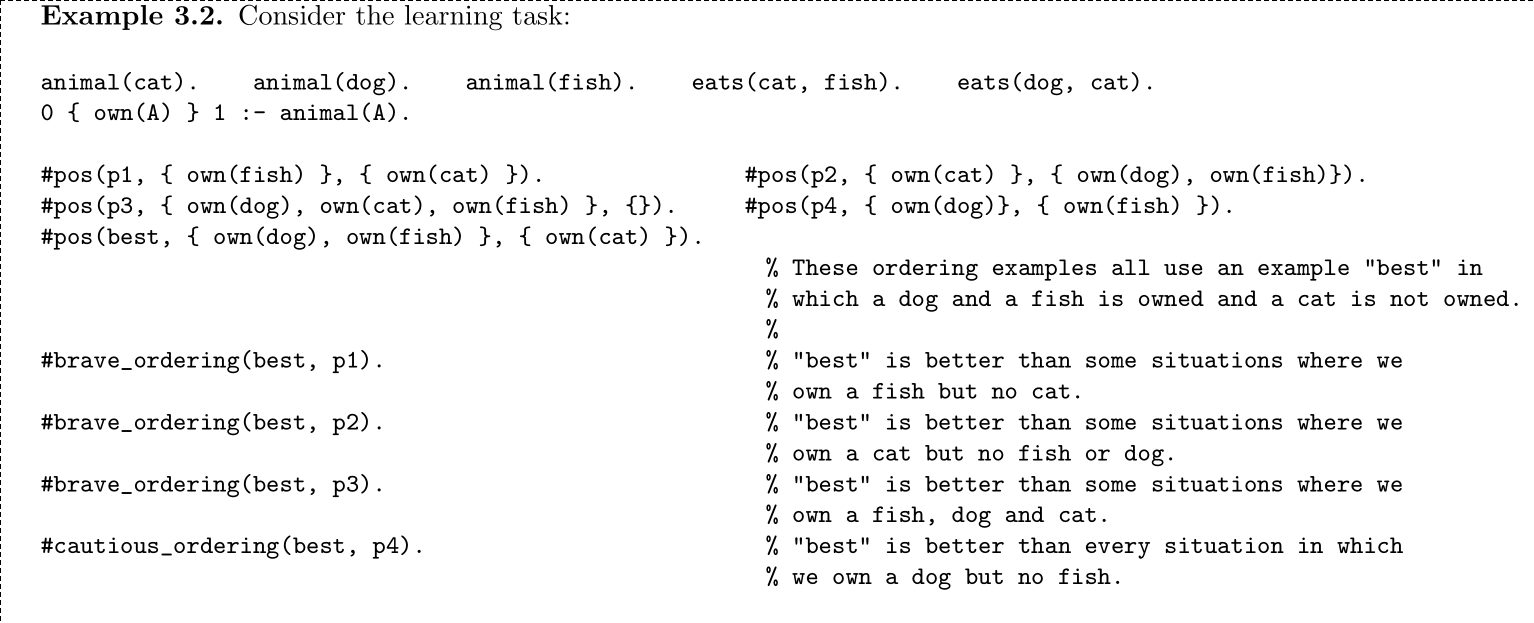
\includegraphics[trim={1.5cm 0.5cm 0.4cm 0.1cm},clip,width=\linewidth]{example_ilasp_1.png}
}
\caption{Sample ILASP program; excerpt from ILASP v3.1.0 manual in \citet{law2017inductive}} 
\end{figure}

\subsubsection{Definitions and Syntaxes}

\begin{description}
    \item [Weak constraint] \hfill \\
    A weak constraint represents an expression of preference in ASP; such that resulting answer sets of a program $P$ can be ranked by preference. Therefore, a weak constraint represents a form of optimization in ASP.
    \item [Partial interpretation] \hfill \\
    A partial interpretation $E$ is a pair of sets of atoms $E^{inc}$ and $E^{exc}$, called the inclusions and exclusions of $E$. We write $E$ as $\langle E^{inc},E^{exc} \rangle$. An answer set $A$ is said to extend $E$ if it contains all of the inclusions ($E^{inc} \subseteq A$) and none of the exclusions ($E^{exc} \cap A = \emptyset$).
    \item [Positive/Negative example] \hfill \\ A positive/negative example is a partial interpretation and can be specified in ILASP as
    \texttt{$\#$pos(example$\_$name,$\left\{e_1^{inc},\ldots,e_m^{inc}\right\},\left\{e_1^{exc},\ldots,e_n^{exc}\right\}$)} or \\
    \texttt{$\#$neg(example$\_$name,$\left\{e_1^{inc},\ldots,e_m^{inc}\right\},\left\{e_1^{exc},\ldots,e_n^{exc}\right\}$)} respectively, \\where \texttt{example$\_$name} is a unique identifier for the example.
    \item [Language bias] \hfill \\
    A language bias in ILASP refers to the search space of possible hypotheses in which inductive solutions should be searched for. These are typically encoded by mode declarations. An example of this is \texttt{$\#$modeo}, which expresses what is allowed to appear in the body of a learned weak constraint.
    \item [Ordering example] \hfill \\ An ordering example is a tuple $o = \langle e_1,e_2 \rangle$, where $e_1$ and $e_2$ are partial (positive-example) interpretations.
    \item [Brave ordering\footnotemark] \hfill \\
    An ASP program $P$ bravely respects $o$ iff $\exists A_1,A_2 \in AS(P)$, such that $AS(P)$ is the answer set of $P$, $A_1$ extends $e_1$, $A_2$ extends $e_2$ and $A_1 \succ_p A_2$.
    \item [Cautious ordering\text{\footnotemark[\value{footnote}]}] \hfill \\
    An ASP program $P$ cautiously respects $o$ iff $\forall A_1,A_2 \in AS(P)$, such that $AS(P)$ is the answer set of $P$, $A_1$ extends $e_1$, $A_2$ extends $e_2$ and $A_1 \succ_p A_2$.
\end{description}

\footnotetext{
\textbf{Note:} Given two positive examples $e_1$ and $e_2$ with identifiers \texttt{id}$_1$ and \texttt{id}$_2$, the ordering example $\langle e_1,e_2 \rangle$ can be expressed in ILASP as \texttt{$\#$brave$\_$ordering(order$\_$name,id$_1$,id$_2$)} or
\texttt{$\#$cautious$\_$ordering(order$\_$name,id$_1$,id$_2$)}, where \texttt{order$\_$name} is an optional identifier for the ordering example.
}

\subsubsection{ILASP Framework}

\justify
\citet{law2017inductive} provides a succinct overview of the ILASP framework to inductively learn hypotheses from answer sets:

\begin{displayquote}
Given an ASP program $B$ called the background knowledge, a set of ASP rules $S$ called the search space and two sets of partial interpretations $E^{+}$ and $E^-$ called the positive and negative examples respectively, the goal is to find another program $H$ called a hypothesis such that:
\begin{enumerate}
    \item $H$ is composed of the rules in $S$ ($H \subseteq S$)
    \item Each positive example is extended by at least one answer set of $B \cup H$ (can be a different answer set for each positive example)
    \item No negative example is extended by any answer set of $B \cup H$
\end{enumerate}
\end{displayquote}

\justify
Similarly, \citet{law2017inductive} provides a framework for extending the above-mentioned method to learn weak constraints from positive examples and ordered answer sets. For brevity, we will exclude the full details of this process; but it is similar to the learning process defined above. For the scope of this project, we will use ordering examples to inductively learn weak constraints. As a result, we will only consider positive examples as partial interpretations.


\subsection{Game Tree}

In order to learn any game strategies, we would first have to conceptualize the concept of a two-player game in a logical and well-computable format. One such useful format would be a game tree. A game tree is a directed graph whose nodes are states of the game and whose edges are action.
% Such that for every node has as many children as legal actions.
The \textit{complete game tree} of a game starts at the initial position and contains all legal actions from each position. 

For this project, we represent such trees using the \texttt{anytree} Python package, which is publicly available in the Python Package Index (PyPI) repository. Given a game tree $T$, we assume the following conventions pertaining to tree objects in the scope of this paper:

\begin{enumerate}
    \item $T(i,j,p,d)$ refers to the node with identifier $j$ present at depth $d$ whose parent node has identifier $i$ at depth $d-1$, where player $p$ is playing the current round.
    \item For cases where no parent node exists, such as for the root node, the following convention will be used: $T(\text{null},j,p,d)$
    \item $i$, $j$ and $d$ defined above all exist in $\mathbb{N}_0$
    \item $d$ has an upper bound of $D$, where $D$ refers to the maximum depth of tree $T$. $d$ corresponding to $0$ would imply the root node.
    \item We will assume that only two players play the corresponding games alternately. As a convention, we will define these players as player $a$ and player $b$. Therefore, $p$ can take the values of $a$ or $b$.
    \item $T(i,j,p,d)[s]$ will refer to the state $s$ of the node $T(i,j,p,d)$. This state contains information on the current configuration of the game and whether the state is terminal. 
    \item $T(i,j,p,d)[a]$ will refer to the action $a$ that was taken to reach the node $T(i,j,p,d)$. Only the root node will have no associated action.
    \item $T(i,j,p,d)[v]$ will refer to the reward value of the node $T(i,j,p,d)$. This will usually only be defined for terminal nodes of a game tree.
    \item $\mathcal{M}(s_0,a_0,\cdots,a_n-1,s_n)$ will refer to a match in the game as a sequence of states. A match can be obtained form a path starting in root node and traversing the tree util a leaf node is reached.
    \item Given a match $\mathcal{M}_a(s_0,a_0,\cdots,a_n-1,s_n)$ we can generate a tree $T_a$ with a single branch rooted in state $s_0$.
    % \item We will work only with \textit{zero-sum games}. This implies that the sum of all rewards is equal to the sum of all losses. Hence, if player $a$ receives a positive reward of $+1$ then player $b$ receives a negative reward of $-1$.
\end{enumerate}

\begin{figure}[H]
    \centering
    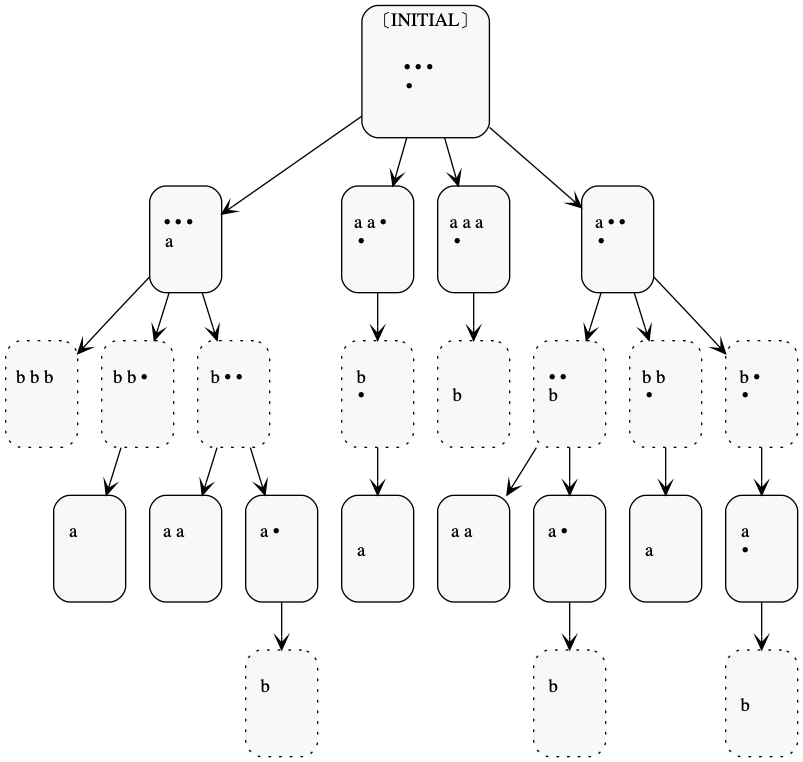
\includegraphics[width=0.85\linewidth]{tree.png}
    \caption{Complete game tree for Nim with initial configuration (3,1,0,0). The actions are represented as part of the nodes instead of the edges.}
\end{figure}
